\chapter{Inledning}

Mängden av producerad data ökar hela tiden, och kräver därför kraftigare och pålitligare
metoder för att hantera datan. Några exempel på helheter som skapar mycket data i form av
dataströmmar är \textit{sakernas internet} (Internet of Things, IoT) system som \textit{smarta städer}
(Smart Cities) där data samlas från sensorer och mobiltelefoner \citep{vakali2014smart}
eller i sjöfart där data samlas från skepp \citep{xu2019internet}. Utvinnande och analysering
av massiva dataströmmar har blivit mera aktuellt i och med nätverksinfrastrukturen förbättras hela tiden.

Inkommande datan  kan oftast inte direkt sparas eller analyseras. Därför är det normalt att
segmentera, filtrera eller gruppera datan före själva analyseringen utförs på datan.
Datan kan också komma från många olika källor \citep{beringer2006online} vilket innebär att datan kräver sammanslagning från källorna. Eftersom mängden data och behovet för analysering av realtidsdata växer
är behovet för robustare arkitekturer för databehandling större. Den här texten fokuserar på metoder för
bearbetning av massiva dataströmmar på arkitekturnivå. Vi går även 
igenom några plattformer som används för distribuerad bearbetning av dataströmmar.

Det finns två olika sätt för behandling av dataströmmar: Lambda-arkitektur 
och Kappa arkitektur. Det visar sig att
båda arkitekturerna har nackdelar. Beroende på vilken man väljer måste man
offra prestation eller komplexitet \citep{mci/Feick2018}.

Avhandlingen beskriver och jämför både Lambda- och Kappa-arkitekturen. Bakgrundskunskaperna
för båda arkitekturerna introduceras i kapitel 2 och 3. I kapitel 5 diskuteras tillfällen där Kappa- 
eller Lambda-arkitektur kan användas.

\section{Använda betäckningar}

I texten används olika betäckningar för att beskriva datastrukturer och deras operationer av dem. Betäckningarna är beskrivna i tabellen nedan.

\begin{tabular}{ |p{3cm}||p{8cm}|  }
 \hline
 \multicolumn{2}{|c|}{Betäckningar} \\
 \hline
 Betäckning & Beskrivning\\
 \hline
  $A$[]   &  En lista med element av typ A \\
 $S$[$a$]   &  Läsoperationen av en lista eller dataström $S$. $a$ är indexet för läsoperationen. Listans värde på indexet $a$ läses. \\
 $(A, B)$   &  En tupel var vänstra värdet är av typ A och högra värdet är av typ B\\
 $S$ & Teckensekvens (eng. string)\\
 \hline
\end{tabular}



\chapter{Introduktion}

Detta kapitel går igenom grunderna för dataströmmar och olika behandligsmetoder av dem. Kapitlet antar att
läsaren kan grunderna i programmering, algoritmer, datanätverk och matematik på kandidatnivå i datavetenskap.

\section{Dataströmmar}

En dataström kan tänkas vara en lista $S$ med $n$ element. Elementen kans läsas från listan med operationen $S$[$t$] 
var $t$ är tidsstämpeln av nutid. Värden kan inte läsas med framtida eller förflutna tidsstämplar. Listan läses
så ofta som möjligt och eventuella värden behandlas sedan. Eftersom datan är i form av en ström kan vissa 
tidsstämplar ge odefinierade värden, som ignoreras. Koden nedan är ett exempel på hur data kan läsas från en
ström. Eftersom $S$[$t$] kan ge odefinierade värden, måste vi säkra att strömmen $S$ innehåller ett värde med
tiddstämpeln $t$ före vi behandlar värdet.

\begin{verbatim}
    while (true) {
      value = S[t]
      if (isDefined(value)) {
        processStreamValue(value)
      }
    }
\end{verbatim}

Datan från dataströmmar kan levereras på många olika sätt. Inom IoT är det normalt att dataströmmar 
levereras över TCP/IP \citep{shang2016challenges}. Dataströmmen kan till exempel behandlas med mjukvara som körs på en server eller ett kluster av många servrar.

\section{Intagning av dataströmmar}

\textit{Intagning} (ingestion) av dataströmmar är processen var data hämtas eller mottags från en extern källa. En paradigm
som kan användas för mottagning av data från källor är publicera-prenumerera -modellen (publish-subscribe, Pub/Sub) \citep{eugster2003many}.
Modellen går ut på ett system som delas in i två grupper, producenter och konsumenter. Konsumenterna prenumererar till kategorier eller mönster
av data som produceras av producenter. Systemet ser till att konsumenterna bara mottar den data dom prenumererar till.

Vi antar att vi har 3 fartyg varav 2 skickar telemetri från fartygets 
kontrollsystem och den den sista telemetri från motorn. Vi har två
olika applikationer, var ena vill behandla telemetri från kontrollsystemet och
andra telemetri från motorn. Publicera-prenumerera -modellen kan användas
effektivt i detta fall. Fartygen som skickar telemetri från kontrollsystemet
kan delas in i en röd grupp och fartygen som skickar telemetri från motorn
kan delas in i en grön grupp, som i bilden nedan [Figur 2.1]. Efter detta kan applikationerna
prenumerera tilla antingen den gröna eller röda gruppen, beroende på hurdan data
dom vill behandla.

\begin{figure}[h]
    \centering
    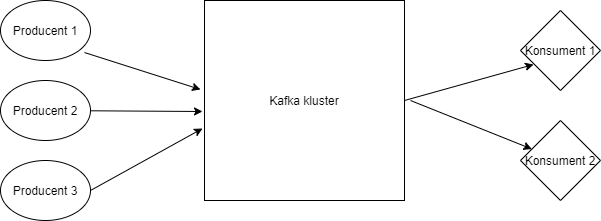
\includegraphics[scale=0.7]{img/prod-cons-model.png}
    \caption{Publicer-prenumerera -modellen med ett Kafka kluster.}
    \label{fig:mesh1}
\end{figure}

\section{MapReduce}
När vi har förmågan att inta data från en dataström behöver vi också ett sätt för att hantera, slå ihop och analysera datan som kommer in. En mycket använd model är den så kallade MapReduce -modellen. MapReduce är en programmeringsmodell som kan bearbeta massiva mängder data på ett kluster av datorer \citep{dean2008mapreduce}. MapReduce baserar sig på två funktioner 
som är bekanta från den funktionella programmerings paradigmen, \textit{map} och \textit{reduce}. Data splittras först i mindre bitar och bitarna ges till MapReduce \textit{arbetare} (workers) som körs på en annan maskin eller process från huvudprocessen. Varje arbetare
kan få en eller flera bitar av datan. Arbetarna kör först funktionen map, som transformerar data och sedan reduce, som slår ihop transformerade data från map -funktionen.

\subsection{Map och Reduce funktionerna}

MapReduce modellens map funktion kan beskrivas som en funktion $f: A \rightarrow B$ var $A = (S, S)$ och $B = (S, K)$ var $K$ är typen av datan som returneras. Map funktionen kan användas för bland annat filtrering,
transformering eller tolkning av serialiserad data.

Vi använder samma scenario i kapitel 2.2 som exempel för att förklara map- och reduce-funktionerna i praktiken. Vi har intagit data från olika fartyg med ett
publicera-prenumerera -system, och sedan sparat det för senare behandling. Vi kon
centrerar oss på data från kontrollsystem, och vi vill beräkna fartygens
medelhastighet. Med map-funktionen kan vi gruppera telemetrin enlight fartyget,
och samtidigt ändra hastighetens enhet från knot till meter per sekund.

\begin{verbatim}
    def map(eventId: S, event: Event): (S, Float) = {
      knotInMetersPerSecond = 0.5144
      emit(tuple(event.shipId, event.shipSpeed * knotInMetersPerSecond))
    }
\end{verbatim}

Map-funktionens parametrar innehåller ett unikt id för händelsen i 
kontrollsystemet och sedan data som fångats under händelsen, i det här fallet
fartygets unika id och hastigheten i knop. Hastighetsenheten ändras till meter
per sekund och värdet anknyts till fartygets id, som används för gruppering av
värden som skapas av map -funktionen.

Efter enhetsomvandligen och gruppering enlight fartyget, kan vi beräkna 
medelhastigheten med reduce.

\begin{verbatim}
    def reduce(shipId: S, speedObservations: Float[]): (S, Float) = {
      result = 0
      for (speed in speedObservations) {
        result = result + speed
      }
      emit(tuple(shipId, result / length(speedObservations)))
    }
\end{verbatim}

Reduce-funktionens parametrar är fartygets id och hastighetsobservationerna 
för fartyget som anknyter sig med farygets id, det vill säga första parametern.
I funktionen summas hastighetsobservationerna ihop och delas sedan med antal
observationer. Funktionen returnerar en tupel med fartygets id och
medelhastigheten för fartyget.

\subsection{MapReduce -processen}

Ett MapReduce program har 7 olika steg. Först splittrats inkommande datan till $N$ segment. Efter splittringen
görs det flera noder av MapReduce programmet var en nod fungerar som \textit{mästare} (master) och andra
som arbetare. Mästarnoden tilldelar arbetarna map eller reduce arbeten. Arbetarna som har som uppgift att utföra map arbeten
läser ett segment som mästarnoden har givit den, kör funktionen map och sparar tupellistan i en buffert i minnet.
Innehållet av buffertarna skrivs under jämna mellanrun till en fil och arbetaren signalerar mästarnoden var datan för en viss
tupel finns i MapReduce klustret. Mästarnoden informerar arbetaren med reduce uppgifter om platser var datan sparad från map skedet
befinner. Datan läses och sorteras sedan så att tuplar med samma nyckel är gruperade tillsammans. Arbetaren kör reduce funktionen på varje
unika nyckel som finns i matade datan. Varje arbetare med ett reduce arbete skriver ut resultatet till en fil. Bilden nedan illustrerar processen.

\begin{figure}[h]
    \centering
    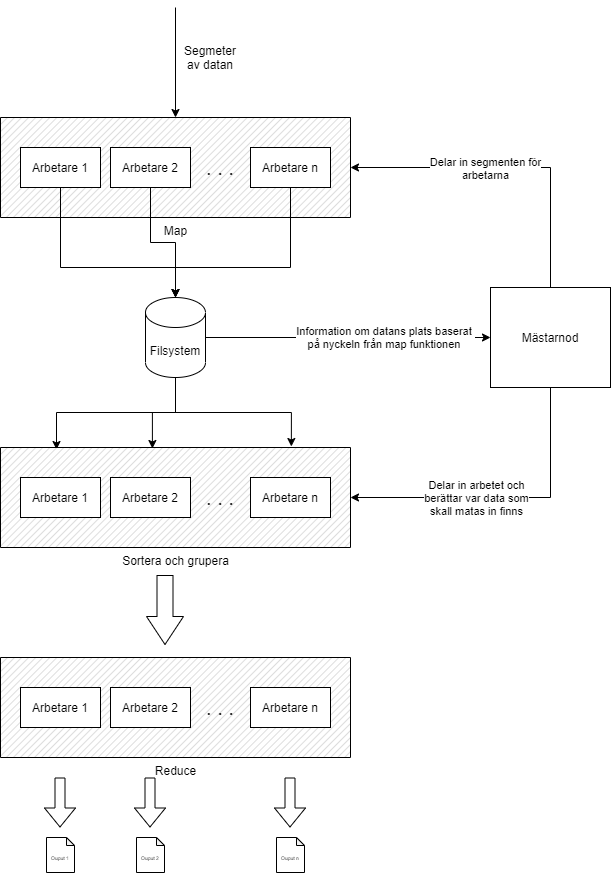
\includegraphics[scale=0.5]{img/map-reduce.png}
    \caption{MapReduce -processen}
    \label{fig:mesh1}
\end{figure}

\chapter{Behandlingsprocesser}

\section{Satsvis behandling av dataströmmar}

\textit{Satsvis behandling} (batch processing) av dataströmmar är en metod för behandling av 
dataströmmar som går ut på att köra behandlingsprogram på datan till exempel mellan jämna
tidsinterval eller när någon viss tröskel arr överskridit \citep{marz2013big}. Satsvisa behandligen
innehåller 3 olika steg. I först steget sparas inkommande datan. Ny inkommande data kan sparas vart
som helst, men det är normalt at använda till exempel Apache Hadoops \textit{distribuerade 
filsystem} (Hadoop Distributed File System). Ny inkommande data sparas i en skild plats från redan
mottagna datan (master data) för att hålla datan oföränderlig under följande steget. I nästa steget processeras datan med till exempel
MapReduce som vi gick igenom i förra kapitlet. Före behandlingen påbörjas slås nya inkommande datan och gamla mottagna datan ihop.
Många olika MapReduce -processer kan köras på datan och resultatet av en MapReduce -process är oftast en vy av något som är
för komplicerat att producera i realtid. Data från behandlingsskedet sparas oftast i en \textit{nyckel-värde} (key-value) databas som sedan kan användas
för att servera datan till olika applikationer. Bilden nedan beskriver satsvisa behandlingsprocessen.

\begin{figure}[h]
    \centering
    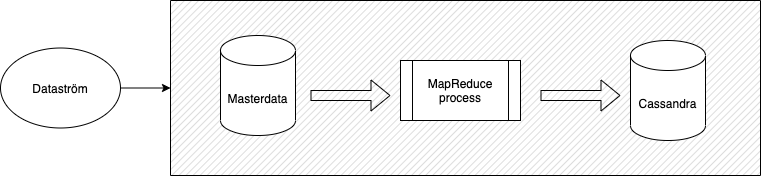
\includegraphics[scale=0.6]{img/batch-pipeline.png}
    \caption{En arkitektursbild av satsvis behandling av dataströmmar. Cassandra används som exempel av en nyckel-värde databas.}
    \label{fig:mesh1}
\end{figure}


\section{Behandling av dataströmmar i realtid}

I vissa fall är satsvisa behandlingen för långsam eftersom vyerna, som representerar behandlad data, måste uppdateras genast när
nya händelser kommer in till systemet \citep{marz2013big}. I stället för att slå ihop gammal
data och ny data och köra en MapReduce -process över all data för att uppdatera vyerna som i 
satsvis behandling, körs behandlingen bara på nya datan och nya vyn slås ihop med gamla vyn.
Eftersom datan kan komma in snabbare än vad det tar för systemet at processera inkommande data
måste köar läggas till före behandlingssekeden för att undvika bortfallning av data. När datan
har kommit igenom kön behandlas den och slås ihop med förra vyn som systemet generera.

\chapter{Platformer för dataströmmar}

\section{Intagning av data med Apache Kafka}

En platform som används ofta för intagning av data Apache Kafka \citep{marz2013big}. Kafka fungerar med publicera-prenumerera -modellen
som beskrevs i kapittel 2.2. \citep{kafka}. Data läses av konsumenter och produceras av producenter [Figur 2.1].

Datan som produceras av producenter i Kafka är \textit{händelser} (events). Händelserna har 3 olika
element: ett nyckelvärde, själva värdet av händelsen och en tidsstämpel. Till exempel, om vi har ett Kafka -kluster som intar telemetri från fartyg på havet så kan nyckelvärdet vara ett unikt nummer som fartyget har i ett datasystem så att händelsen kan kopplas samman med information av fartyget, värdet är kursen av fartyget och tidsstämpeln tiden när fartyget har skickat händelsen.

Kafka ger också möjligheten att dela in händelser i olika kategorier som kallas \textit{ämnen} (topics). Konsumenterna prenumererar till olika ämnen och får händelser från prenumererade ämnen.

\section{Behandling med Apache Storm}

Apache storm är ett distribuerat beräkningssystem \citep{apachestorm}. Apache Storm är gjort för att utföra arbeten
på samma sätt som i MapReduce, men göra dem i realtid och inte satsvist. Storm har några huvudkonsept: \textit{Topologier} (topologies),
\textit{strömmar} (streams), \textit{kranar} (spouts) och \textit{bultar} (bolts).
\begin{itemize}
    \item \textbf{Topologier} definierar hela strukturen av systemet. Topologier i Storm kan tänkas vara en graf av bultar och kranar.
    \item \textbf{Strömmar} är liknande till definitionen av dataströmmar som gavs tidigare. Strömmarna i Storm är sekvensser med tuplar som kan innehålla till exempel teckensekvenser eller heltal.
    \item \textbf{Kranar} i Storm är källan till en
eller flera strömmar. Kranar läser oftast data från en utomstående källa, till exempel ett Apache Kafka kluster, och avsänder dom till Storms topologi. Kranarna kan vara 
\textit{pålitliga} (reliable) var inkommande datan sparas och kan avsändas igen i fall något fel uppstår eller \textit{opålitliga} (unreliable)
var datan inte sparas.
   \item \textbf{Bultarna} sköter själva behandlingen av datan som kan vara i form av filtrering, sammanfattning, transformering 
eller sammanslagning. Bultarna prenumererar till en eller flera Storm strömmar varifrån bulten läser inkommande data. Färdiga datan från
bultarna kan skickas till en eller flera Storm strömmar.
\end{itemize}

Storm bultarna och kranarna körs på såkallade \textit{uppgifter} (tasks). Uppgifterna körs på egna trådar på en kluster av maskiner 
för att undvika blokering av andra uppgifter. Topologierna körs på en eller flera arbetarprocesser. Arbetarprocesserna kan till exempel vara
skillda processer på en maskin eller ett kluster av maskiner. En Storm grupering har 3 olika delar\citep{marz2013big}: Nimbus, Apache ZooKeeper 
kluster och Storm kluster. Nimbus är en mestarnod som ser till att topologin fungerar på rätt sätt och ger upfigter till arbetaren, ZooKeeper
används för at överse och orkestrera topologin och Storm klustret innehåller själva arbetarna. Varje nod med arbetare i storm klustret har en nod
som handleder andra arbetarnoderna. Handledaren tar kommandon från Nimbus och delegerar dem sedan framåt till arbetarnoderna.

Storm har ett system för pålitlighet som konstant granskar att tuplarna från strömmarna processeras i Storm topologin. Om en bult överskrider en
viss tidströskel under behandlingen så avbryts behandlingen av tupeln. Behandlingen av den obehandlade tupeln provas igen senare.

Figur 4.1 beskriver hur dataströmmsbehandling i realtid kan genomföras
med Apache Storm.


\begin{figure}[h]
    \centering
    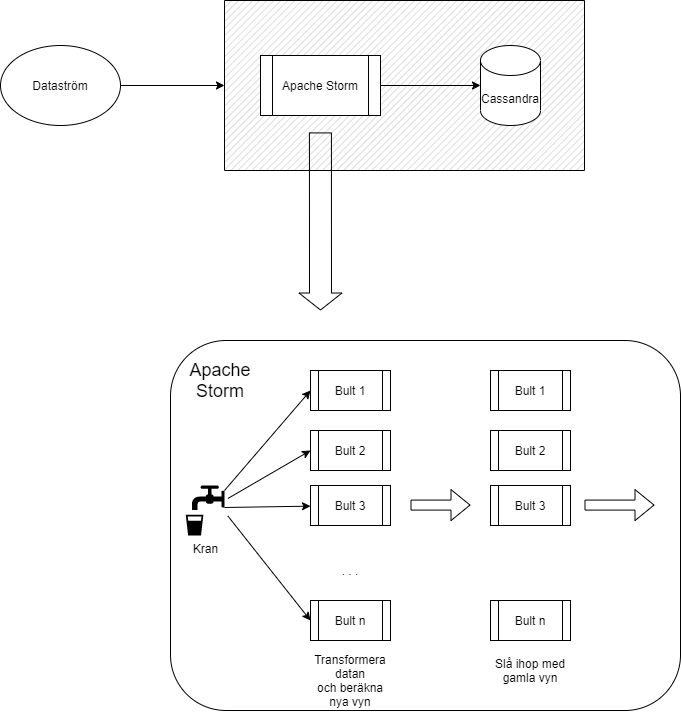
\includegraphics[scale=0.7]{img/speed-layer.png}
    \caption{Behandling av dataströmmar i realtid med Apache Storm. Cassandra som exempel av en nyckel-värde databas.}
    \label{fig:mesh1}
\end{figure}


\chapter{Arkitektur}

\section{Lambda-arkitektur}

Lambda-arkitekturen är en arkitektur som kombinerar satsvis och   
realtidsbehandling av dataströmmar \citep{marz2013big}. Lambda-
arkitekturen kan tänkas ha 2 \textit{nivåer} (layers) var data 
behandlas på olika sätt. 

Första nivån kallas \textit{realtidsnivån} 
eller \textit{fartnivån} (speed layer). Realtidsnivån behandlar 
inkommande data direkt för att ge snabba resultat och insikter till 
slutanvändaren. Första nivån behandlar datan med snabba algortimer som
skalar lineärt eller logaritmiskt med mängden data, eftersom realtidsnivån 
inte tål långa behandlingstider. Inkommande datan måste dock köas
före behandlingen eftersom det aldrig är garanterat att datan kan behandl
as direkt. Behandlingen kan basera sig på ett MapReduce system.

Andra nivån kallas satsvisa nivån
soms uppgift är att köra beräkningsvis komplexa algoritmer på inkommande
data, till exempel träning av neuron nätverk. Satsvisa nivån kan också användas för att
köra behandlingsarbeten på tidigare data i stället för inkrementell behandling som
i realtidsnivån. Inkommande datan sparas oftast i en databas före satsvisa processen 
körs på datan.

Lambda-arkitekturen kan genomföras var som hälst, men det är normalt att bygga 
arkitekturen på \textit{molntjänster} (cloud service)\citep{kiran2015lambda}. Kiran et 
al. går igenom olika alternativ för att genomföra lambda-arkitektur i molntjänster
med hjälp av effektiv användning av molntjänstens olika platformer. Lambda-arkitekturen
kan också genomföras delvis i molnet och delvis lokalt eller på \textit{kanten} (edge) \citep{yamato2016proposal}.
Behandling på kanten betyder att data kan behandlas redan på sensorns hårdvara i stället
för att data behandlas centralt på en server. Yamato et al. föreslår ett sätt där
kantnoderna sparar data i en egen databas och updaterar analytiska modeller. Data
förflyttas satsvist över till molnet under natten.

Figur 5.1 beskriver Lambda-arkitekturens uppbyggnad.

\begin{figure}[h]
    \centering
    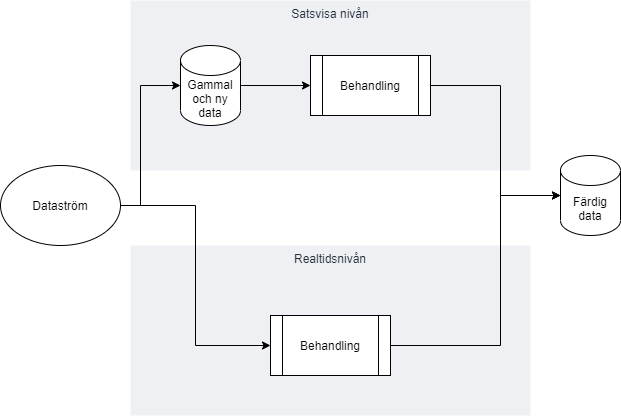
\includegraphics[scale=0.7]{img/lambda-arch.png}
    \caption{Lambda-arkitektur.}
    \label{fig:mesh1}
\end{figure}

\subsection{Exempel}

Vi går igenom hur lambda-arkitekturen skulle se ut i exempelfallet vi
användt i kapitel 2. I kapittel 2.3 demonstrerade vi MapReduce -processen
med ett exempel var vi vill mäta fartygens medelhastighet. Eftersom medelhastigheten
kan beräknas på nytt utan att vi behöver tillgång till gamla fartobservationer, kan 
medelhastighetsberäkningen göras på realtidsnivån med en liknande MapReduce -process.
Nya reduce-funktionen ser ut på följande sätt:

\begin{verbatim}
    def reduce(shipId: S, speedObservations: Float[]): (S, Float) = {
      newSpeedObservation = speedObservations[0]
      oldObservationsSum = getOldMean(shipId) * amountOfObservations(shipId)
      emit(
        tuple(
          shipId,
          (oldObservationsSum + newSpeedObservation) / amountOfObservations
        )
      )
    }
\end{verbatim}

Vi behöver tidigare medelhastigheten och mängden observationer för fartyget för att
beräkna nya medelhastigheten. Vi kan hämta tidigare medelhastigheten med hjälp av
funktionen \textit{getOldMean} med fartygets id som parameter. Mängden observationer
kan hämtas med funktionen \textit{amountOfObservations} med fartygets id som parameter.

Vi vill träna en linjär regressionsmodell av fartygens hastigheter. Linjär regression
kan inte tränas inkrementellt, så vi måste träna modellen på tidigare data och ny data.
Detta kan göras med hjälp av satsvisa nivån. Inkommande hastighetsobservationer sparas i
en databas som också innehåller data på hastigheter från hela operationstiden av 
systemet. Satsvisa behandlingen är en MapReduce -process som körs en gång per dag. När
satsvisa arbetet börjar, läses hela databasen in till MapReduce -processen som sedan
tränar en linjär regressionsmodell på basis av ny data som kommit in under pågående dag
och gammal data från tidigare dagar.


\section{Kappa-arkitektur}

Kappa-arkitekturen kan tänkas som Lambda-arkitekturen utan satsvisa 
nivån \citep{kappa}. Kappa koncentrerar endast på behandling av data i realtid och
försöker ta bort komplexitet från Lambda-arkitekturen. Ett problem med 
Lambda-arkitekturen är att den kan värka överdriven för vissa problem, och onödig
kompleksitet resulterar i underhåll av onödig kod. Om behandlingen som görs
på data är enkel, till exempel summande av ord från en dataström av meningar,
behövs det inte en nivå för satsvis behandling eftersom summande kan bra göras
på realtidsnivån. Kappa-arkitekturen kan vid behov transformeras till 
Lambda-arkitektur med att lägga till en satsvis nivå.

Kappa-arkitekturen genomförst oftast med hjälp av någon platform. Till exempel
Twitter genomför Kappa-arkitekturen med deras egna platform \citep{yang2018robust}
och Zschornig et al. använder Apache Kappa och föreslår ett sätt var 
Kappa-arkitekturen kan genomföras på \textit{mikrotjänster} (microservices), altså små applikationer som körs i isolation från varandra.
\citep{zschornig2017personal}. Kappa-arkitekturen kan utplaceras var som hällst är,
men det ärnormalt att Kappa-arkitekturen utplaceras i en molntjänst.

Figur 5.2 visar hur data går igenom Kappa-arkitekturen. Före behandlingsprocessen
finns en kö som ser till att inkommande data inte faller bort när behandlingsprocessen är upptagen med behandling av tidigare data.

\begin{figure}[h]
    \centering
    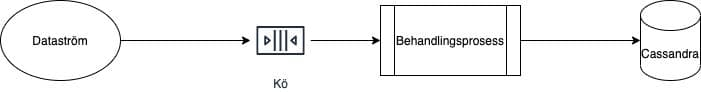
\includegraphics[scale=0.8]{img/kappa-arch.jpg}
    \caption{Kappa-arkitektur. Cassandra används som en databas för att spara behandlad data.}
    \label{fig:mesh1}
\end{figure}

\section{Jämförelse av arkitekturerna}

Fast Lambda-arkitekturen kan tänkas vara en utvidgning av Kappa-arkitekturen,
finns det ändå användningsfall var den ena fungerar bättre än den andra. Om
applikationen kräver till exempel maskininlärning i ett tidigt skede av utväcklingen så är
Lambda-arkitekturen ett bättre alternativ eftersom den redan innehåller möjlighheten för satsvis behandling. I alla andra fall är det bra att välja
Kappa-arkitekturen, fast den inte är lika omfattande som Lambda-arkitekturen på grund av att satsvisa nivån fattas. Med Kappa-arkitekturen undviker man upprätthållning av potentiellt onödig kod och Kappa skalar lätt till en arkitektur
som är lika robust som Lambda-arkitekturen.

\chapter{Slutsatser}

I denna avhandling har vi gått igenom två olika arkitekturer som kan användas för
behandling av massiva dataströmmar. Vi har även gått igenom underliggande koncept
och några platformer som kan användas.

Kappa- och Lambda-arkitekturerna har olika användningsfall, men Kappa-arkitekturen
kan oftast tänkas som den nödvändigare arkitekturen eftersom den skalar lätt till
samma förmågor som Lambda-arkitekturen. Lambda-arkitekturen kan vara i flera
applikationer för komplext och jobbigt att upprätthålla.

Även om behandling av massiva dataströmmar är ett mycket aktuellt ämne, finns det
relativt lite metoder och arkitekturer för problemet. Dessutom kommer framtiden
kräva nya variationer av Kappa- och Lambda-arkitekturen för att kunna behandla en
konstant växande mängd data.
